% !TeX root = ..\main.tex
\section{Kiến trúc hệ thống}
\subsection{Tổng quan}
\begin{figure}[!htp]
	\centering
	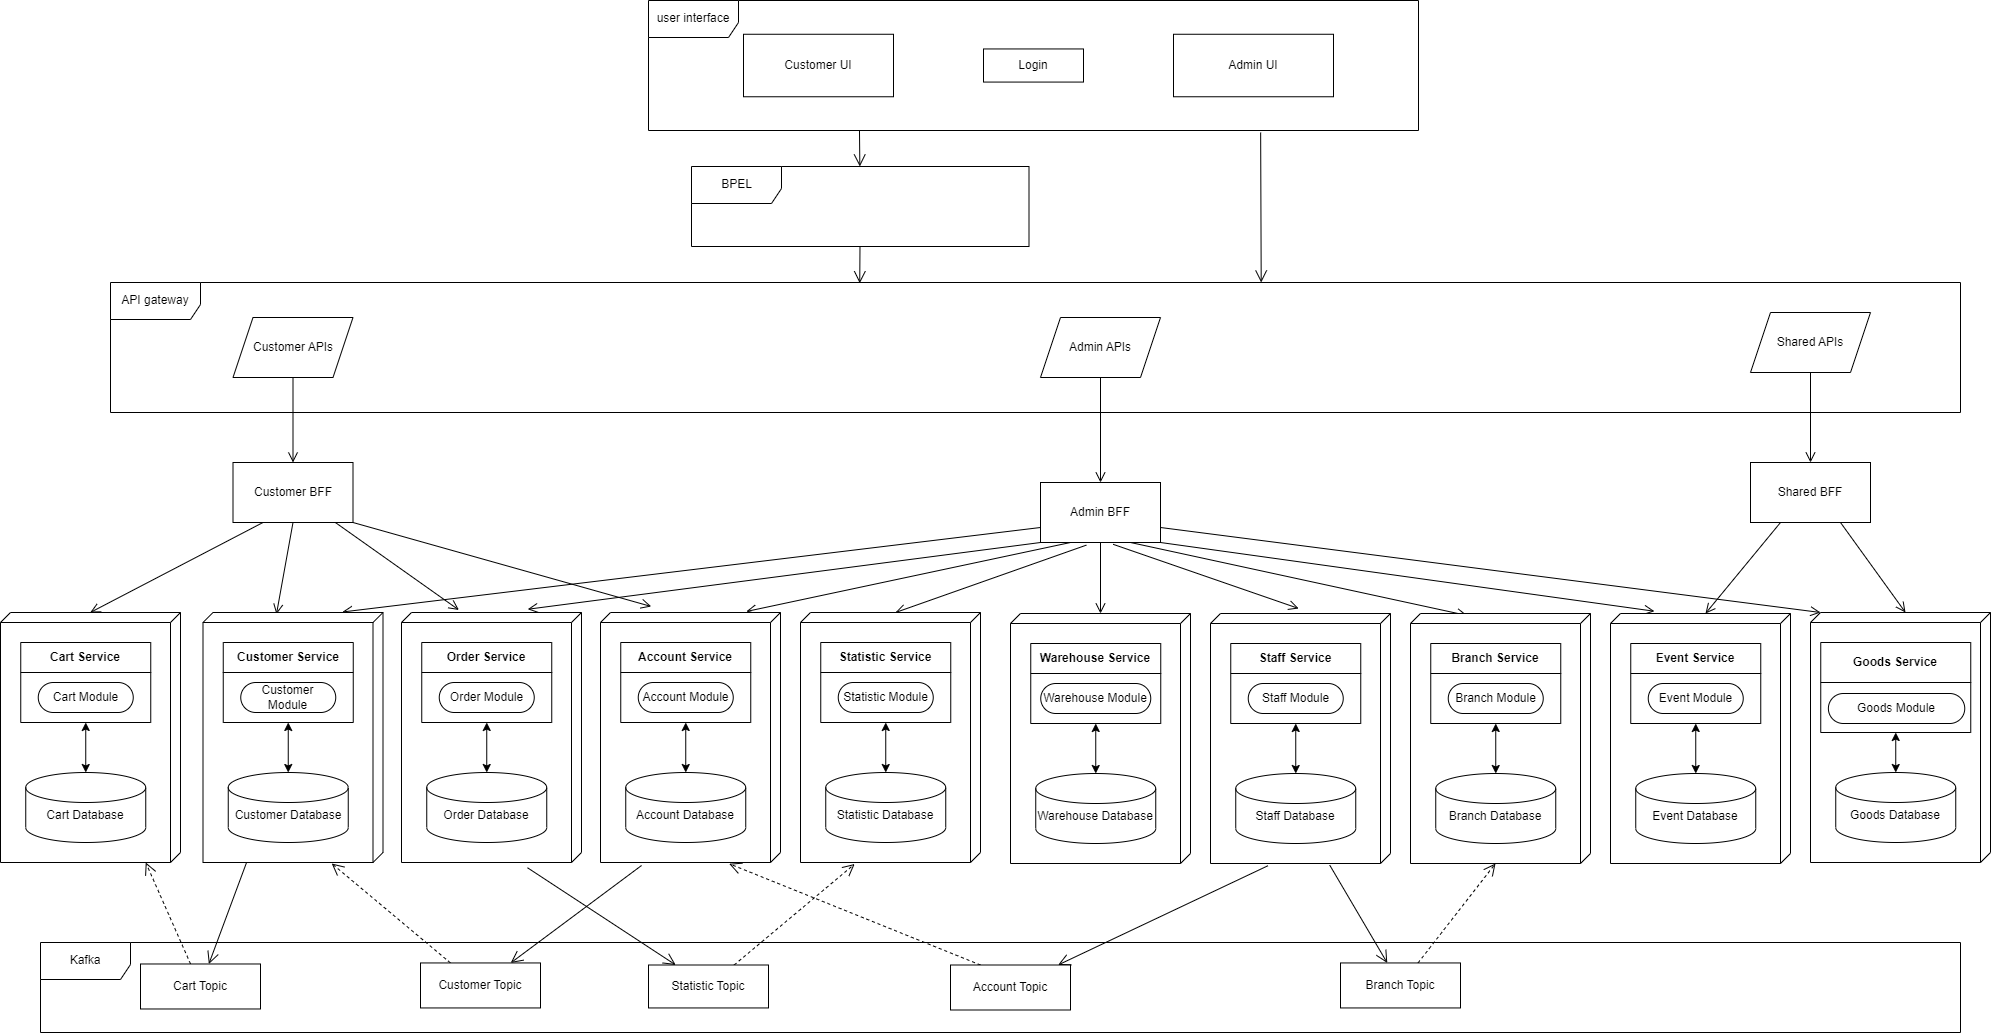
\includegraphics[width=6in]{img/Architecture/general-architect.png}
	\newline
	\caption{Tổng quan kiến trúc hệ thống}
\end{figure}

\subsection{Tầng UI}




\subsubsection{CustomerUI}
Module này bao gồm các class dùng để hiển thị UI đối với phía khách hàng
\begin{figure}[!htp]
	\centering
	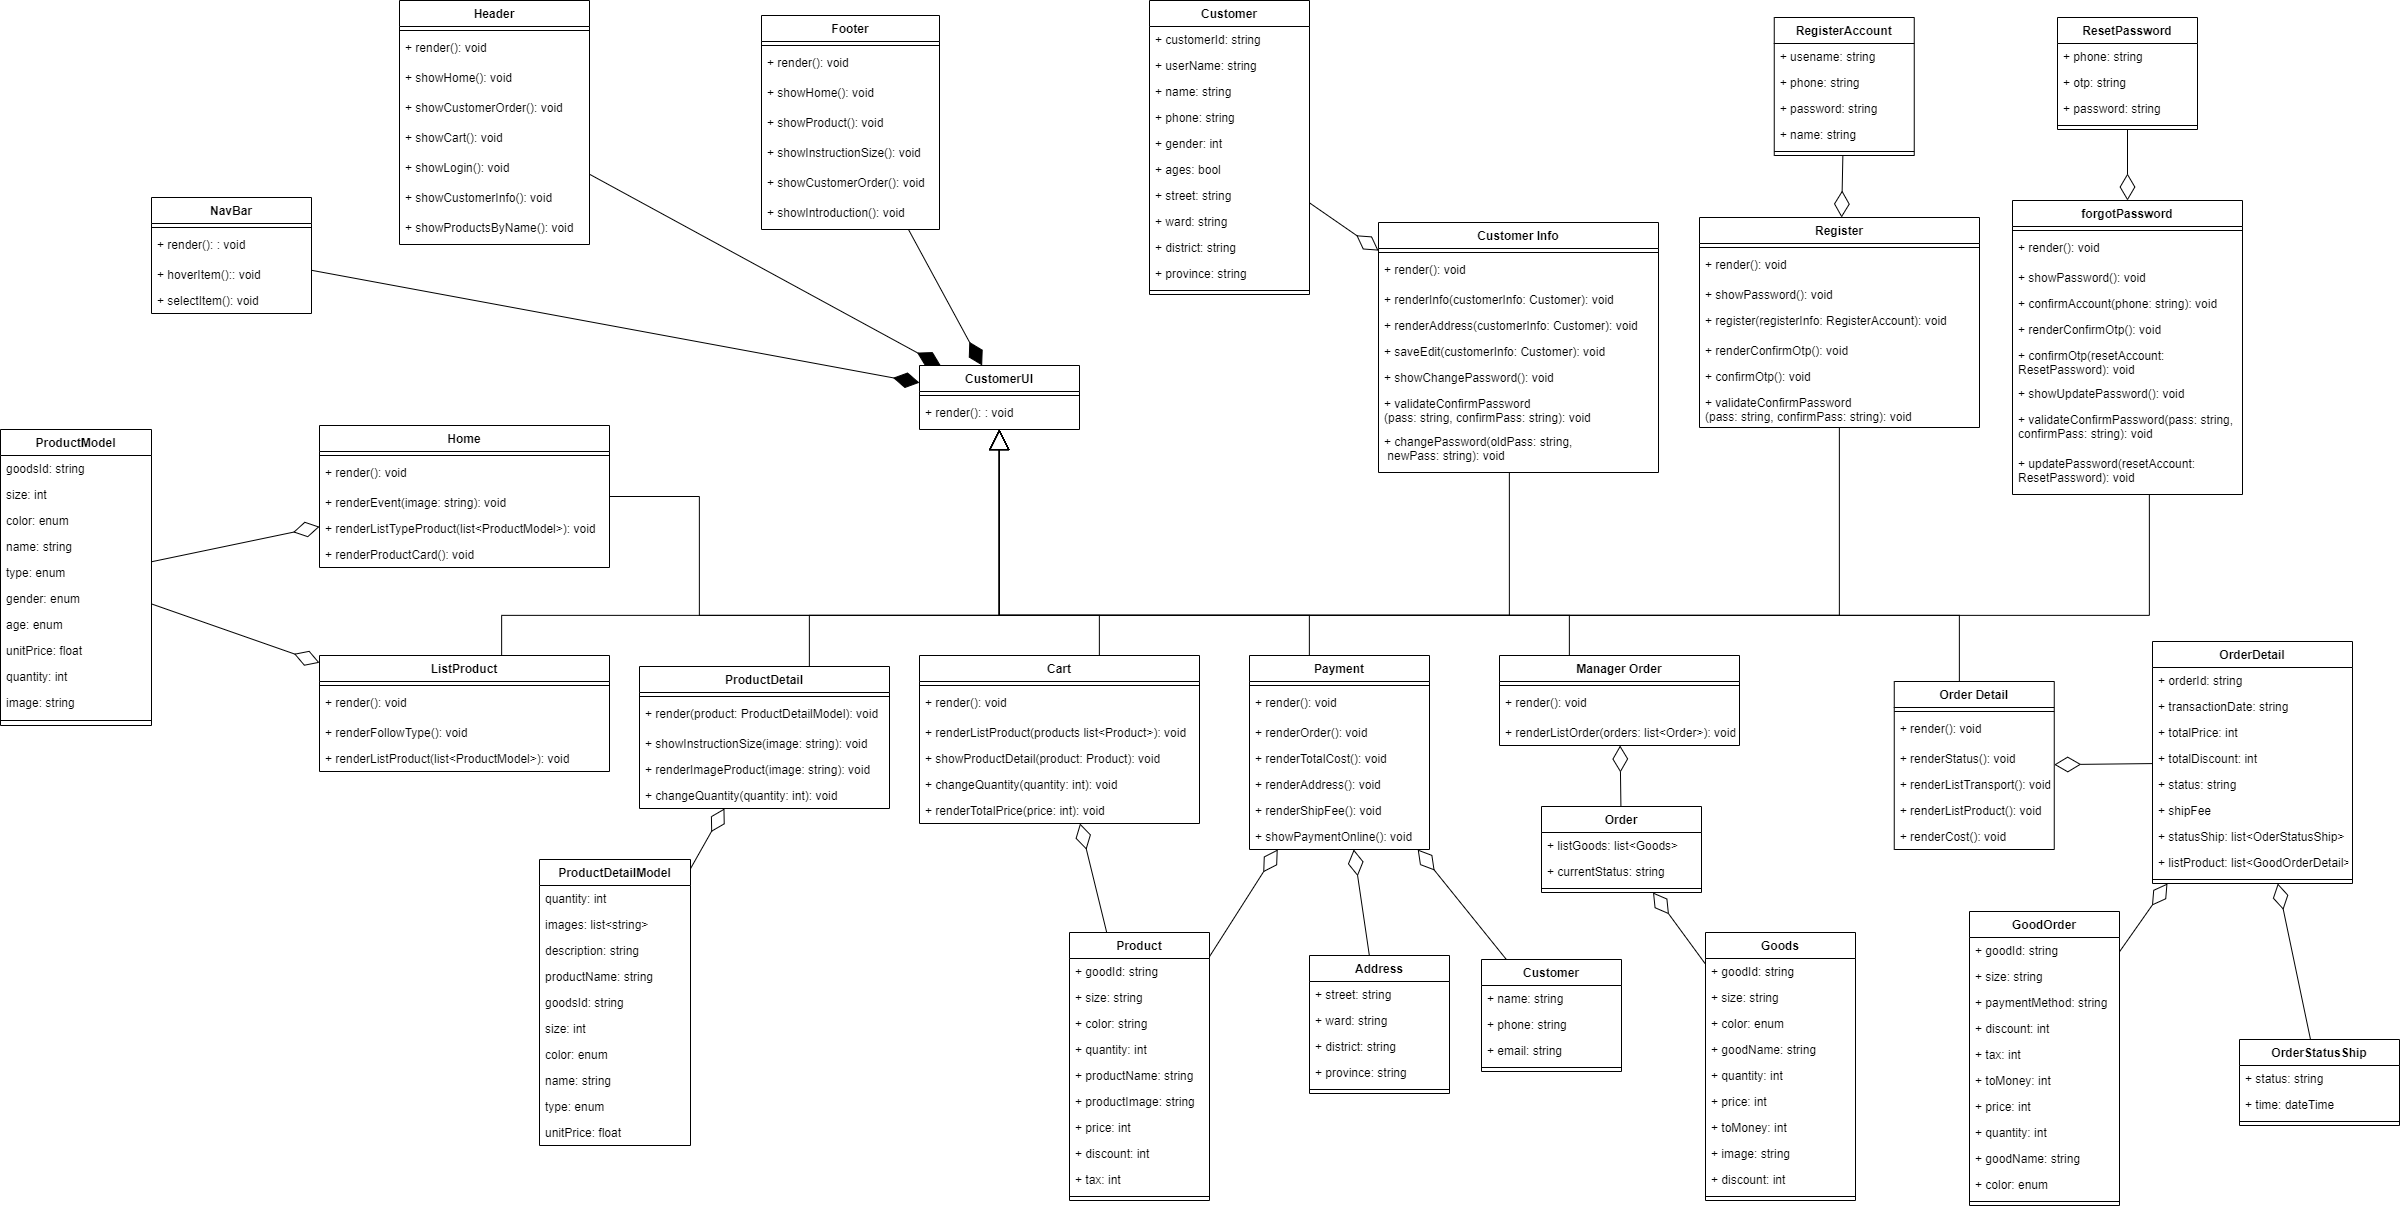
\includegraphics[width=17cm]{img/Architecture/UI/customer UI.png}
	\newline
	\caption{Lược đồ class của Module CustomerUI}
\end{figure}
\textbf{Mô tả:}
\begin{quote}
	\begin{itemize}
		\item CustomerUI
		\item NavBar
		\item Header
		\item Footer
		\item ..
	\end{itemize}
\end{quote}

\subsubsection{LoginUI}
LoginUI là một class dùng để hiển thị trang đăng nhập cho cả phía khách hàng và quản trị viên
\begin{figure}[!htp]
	\centering
	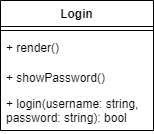
\includegraphics[width=2cm]{img/Architecture/UI/loginUI.png}
	\newline
	\caption{Lược đồ class của LoginUI}
\end{figure}
\textbf{Mô tả:}
\begin{quote}
	\begin{itemize}
		\item CustomerUI
		\item NavBar
		\item Header
		\item Footer
		\item ..
	\end{itemize}
\end{quote}

\subsubsection{AdminUI}
Module này bao gồm các class dùng để hiển thị UI đối với phía quản trị viên

\begin{figure}[!htp]
	\centering
	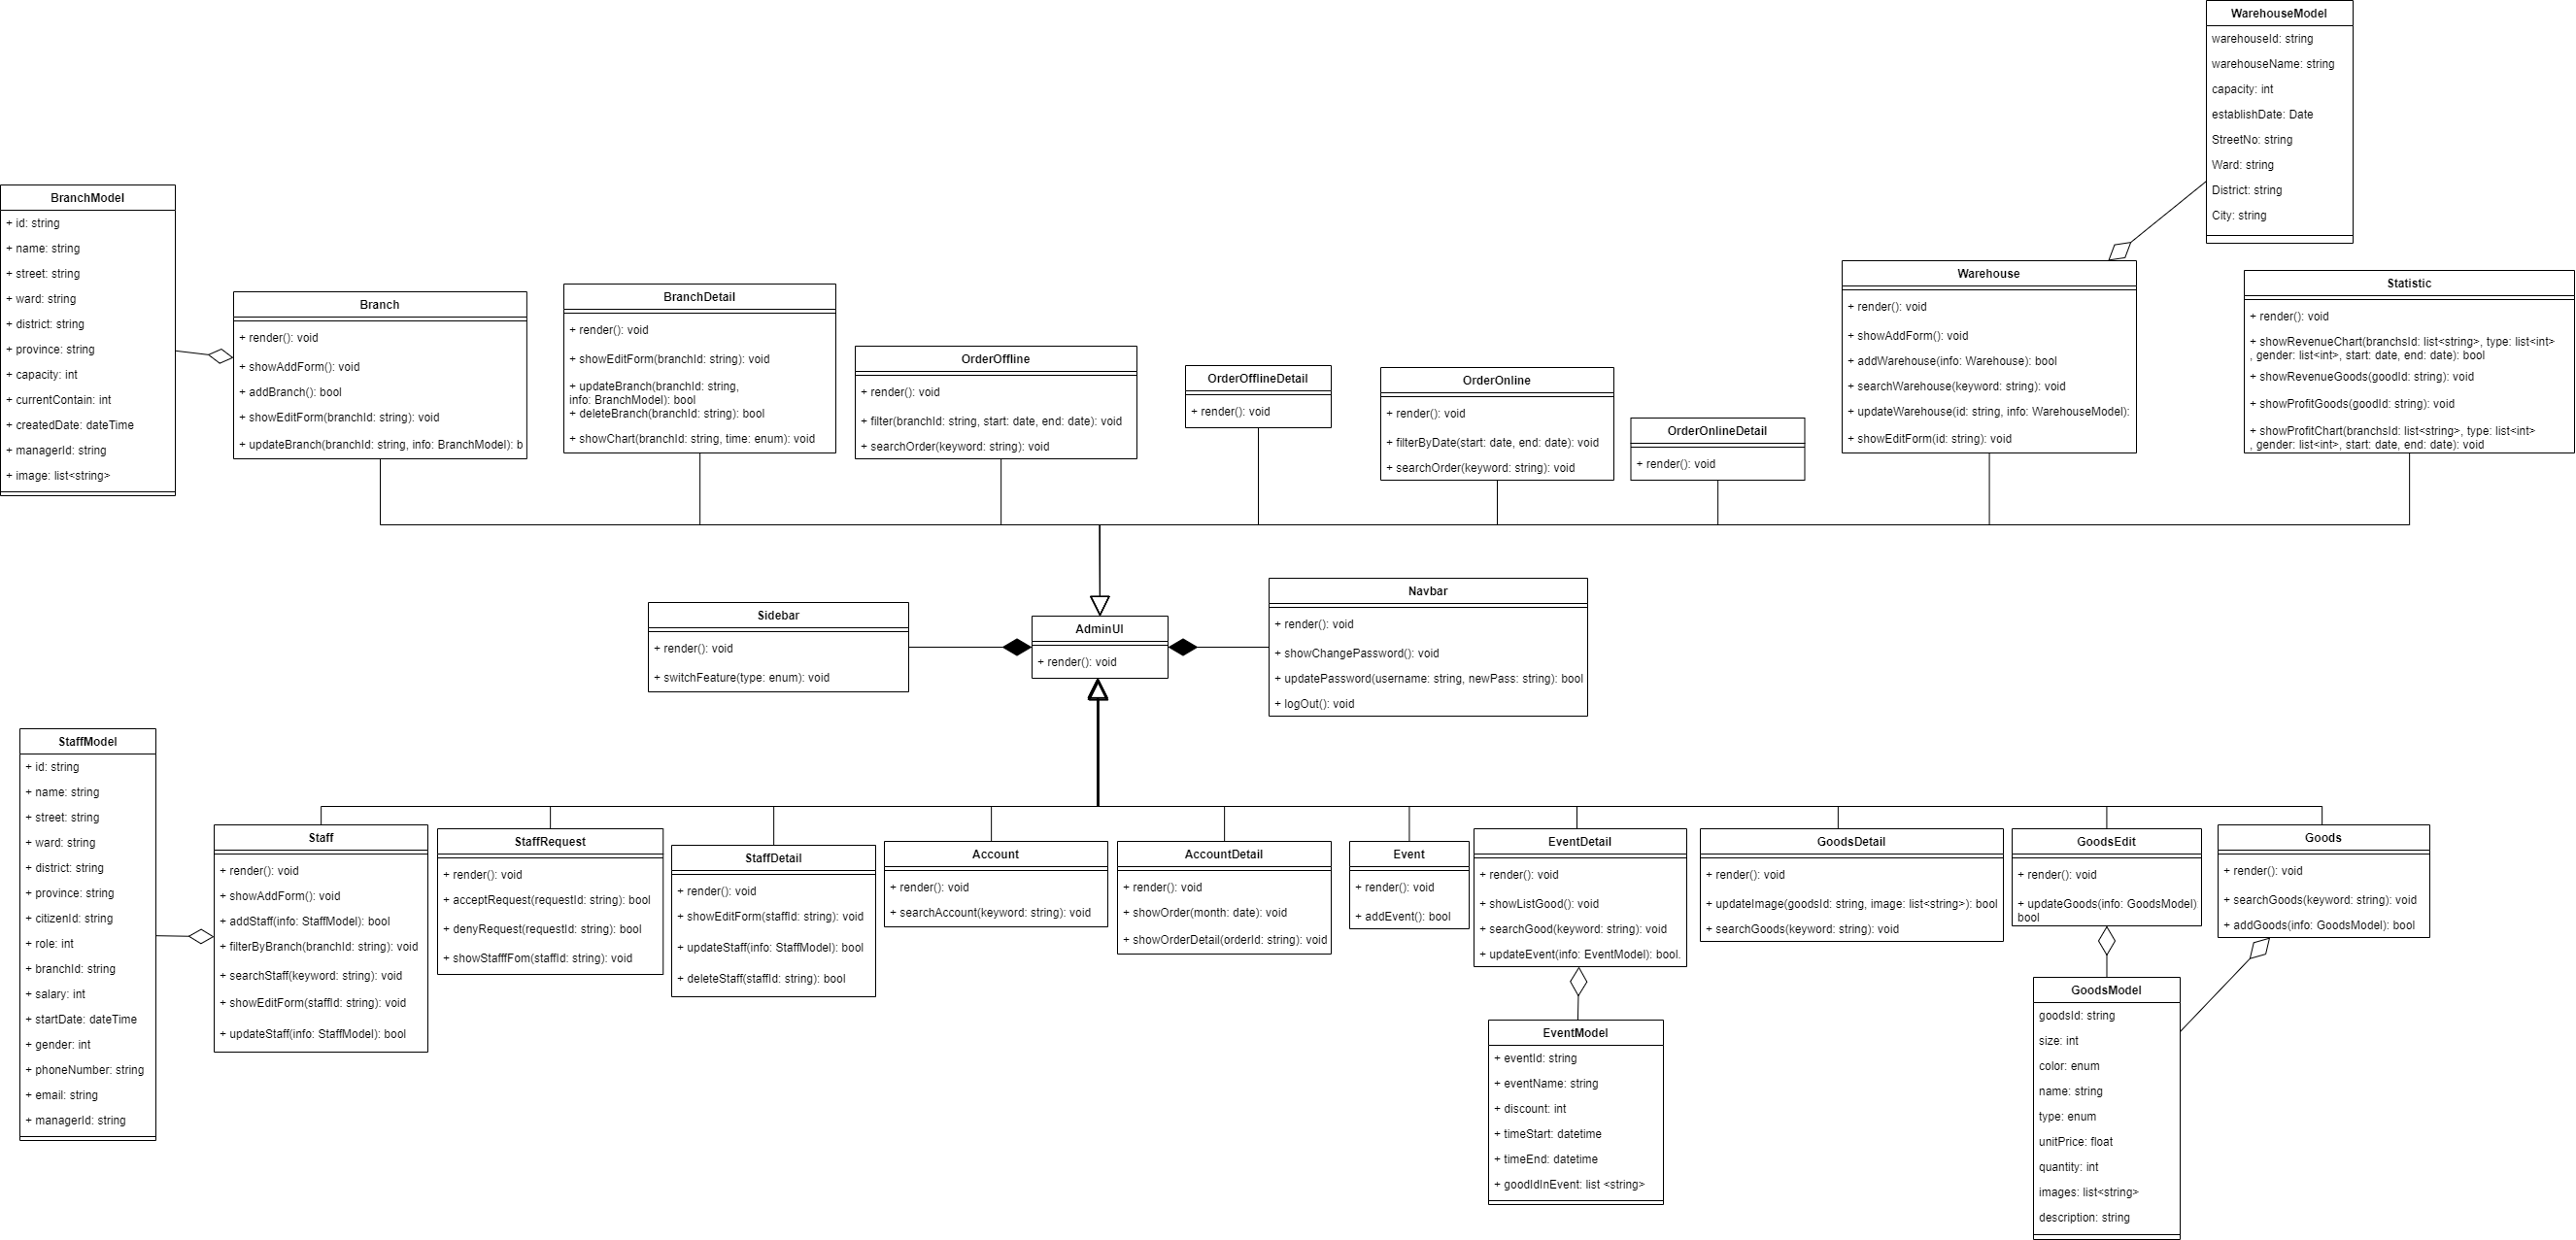
\includegraphics[width=17cm]{img/Architecture/UI/adminUI.png}
	\newline
	\caption{Lược đồ class của Module AdminUI}
\end{figure}
\textbf{Mô tả:}
\begin{quote}
	\begin{itemize}
		\item CustomerUI
		\item NavBar
		\item Header
		\item Footer
		\item ..
	\end{itemize}
\end{quote}





\subsection{Tầng API}
\subsubsection{Customer APIs}
Module này dùng để chứa các API được xuất ra ngoài cho phía khách hàng

\subsubsection{Admin APIs}
Module này dùng để chứa các API được xuất ra ngoài cho phía quản trị viên

\subsubsection{Shared APIs}
Module này dùng để chứa các API được xuất ra ngoài cho bất kì đối tượng người dùng nào




\subsection{Tầng service}

Lược đồ class ở tậng service được xây dựng theo các thành phần sau:
\begin{itemize}
	\item Repository: Class dùng để truy cập trực tiếp đến dữ liệu trong Database
	\item Model: Class dùng để chứa thông tin nhận lên từ Database
	\item Controllers: Class dùng để xử lý các logic nghiệp vụ
	\item Response: Class chứa thông tin trả về khi có yêu cầu từ bên ngoài
	\item Các Interface: Giúp đảm bảo nguyên lý \textbf{Dependency inversion principle} của \textbf{SOLID}
	      \begin {itemize}
	\item IRepository: Cung cấp các api cho các class Controller
	\item IController: Cung cấp các api để bên ngoài service truy cập đến
\end{itemize}
\end{itemize}



\subsubsection{Customer Order Service}
\begin{figure}[!htp]
	\centering
	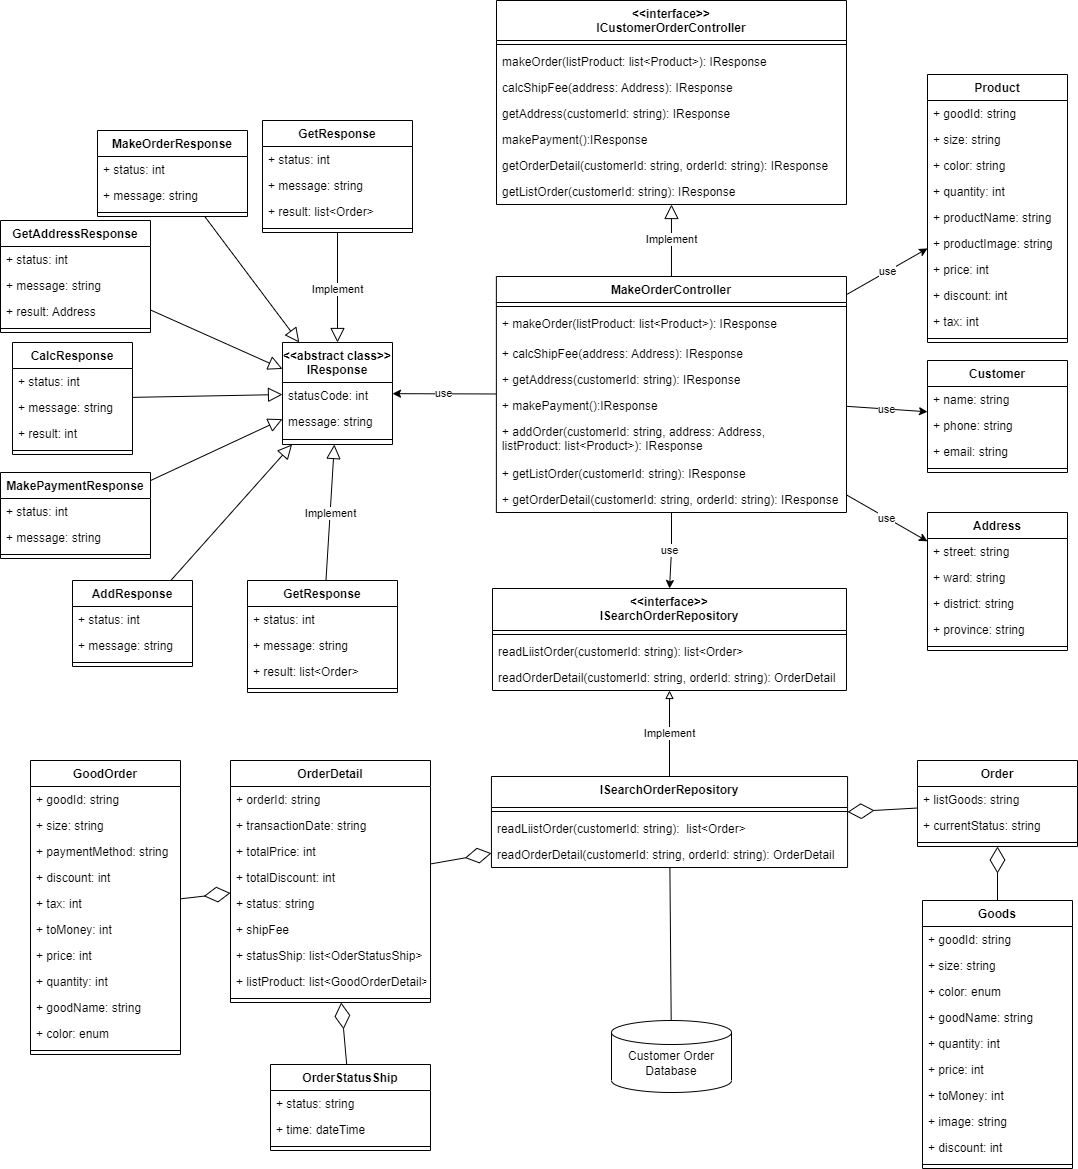
\includegraphics[width=13cm]{img/Architecture/service/CustomerOrderService.png}
	\newline
	\caption{Lược đồ class của Customer Order Service}
\end{figure}



\subsubsection{Cart Service}
\begin{figure}[!htp]
	\centering
	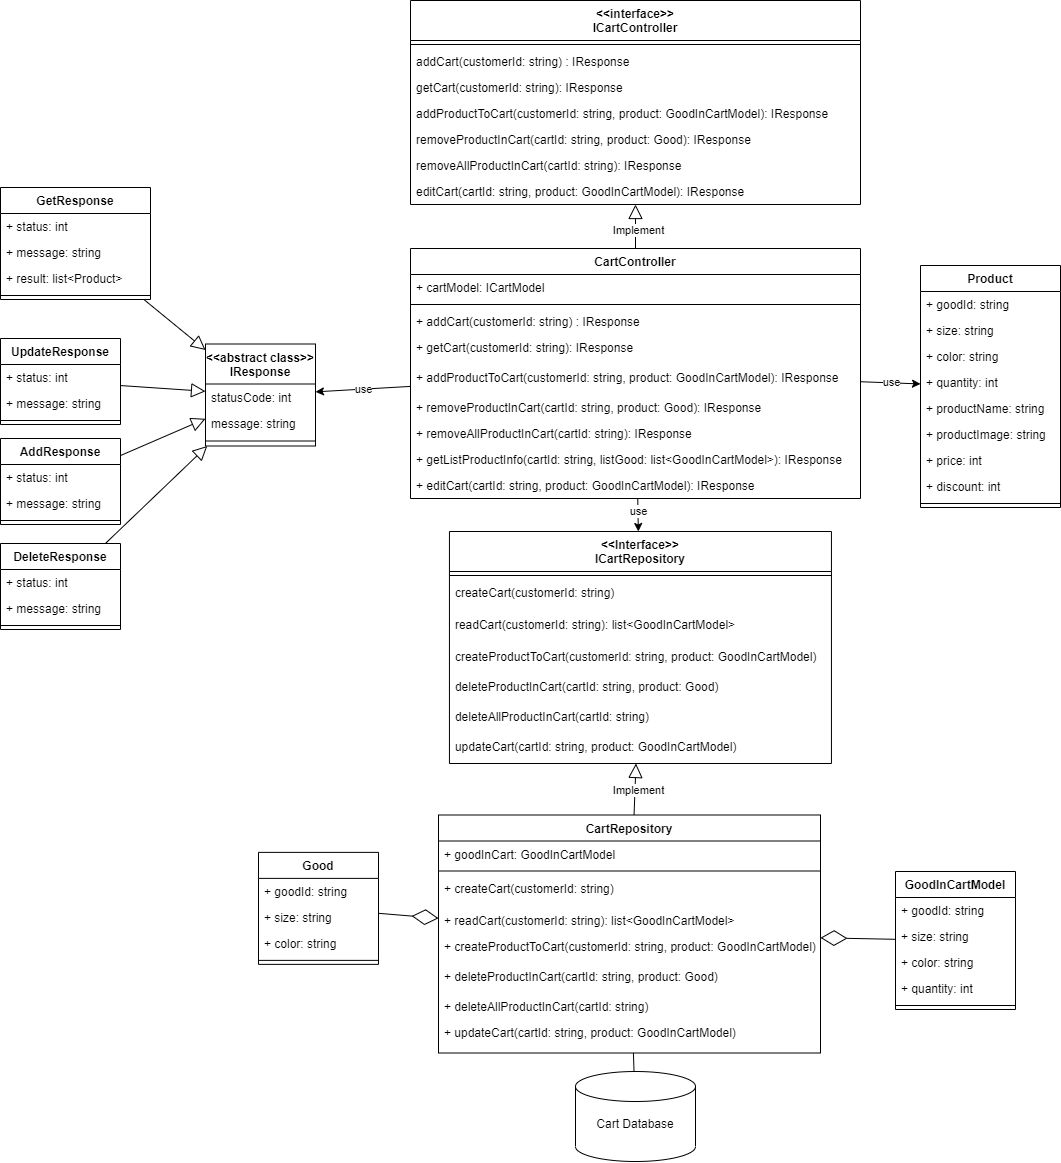
\includegraphics[width=11cm]{img/Architecture/service/CartService.png}
	\newline
	\caption{Lược đồ class của Cart Service}
\end{figure}


\subsubsection{Customer Service}
\begin{figure}[!htp]
	\centering
	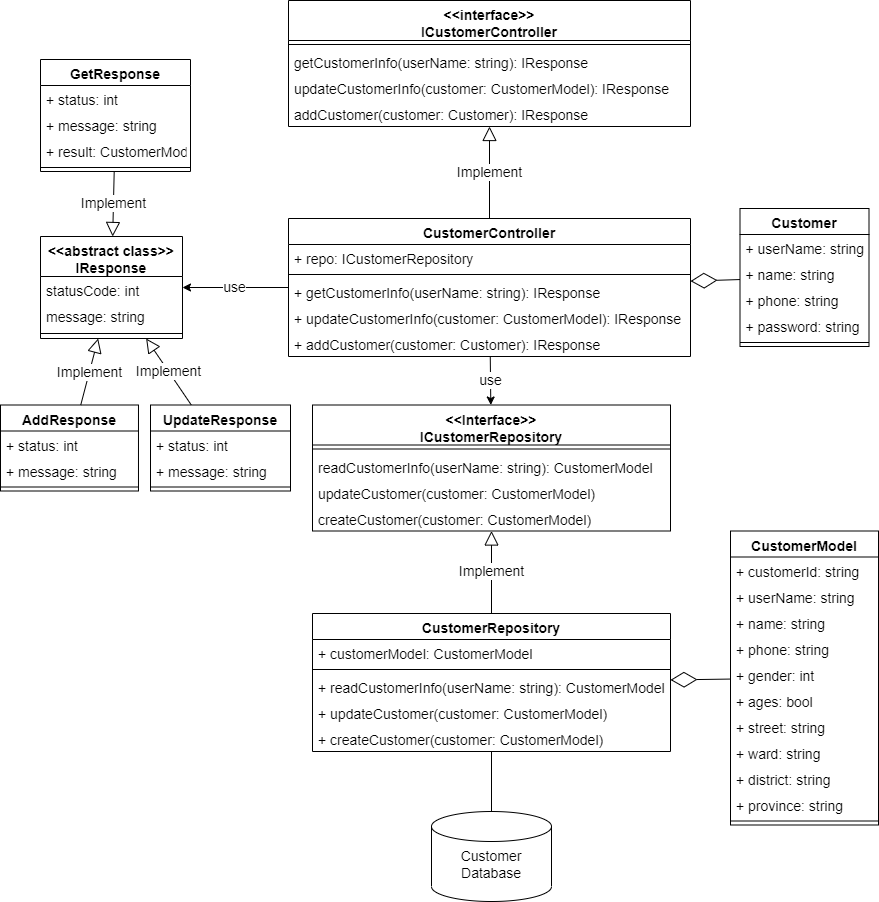
\includegraphics[width=11cm]{img/Architecture/service/CustomerService.png}
	\newline
	\caption{Lược đồ class của Customer Service}
\end{figure}



\subsubsection{Order Service}
\begin{figure}[!htp]
	\centering
	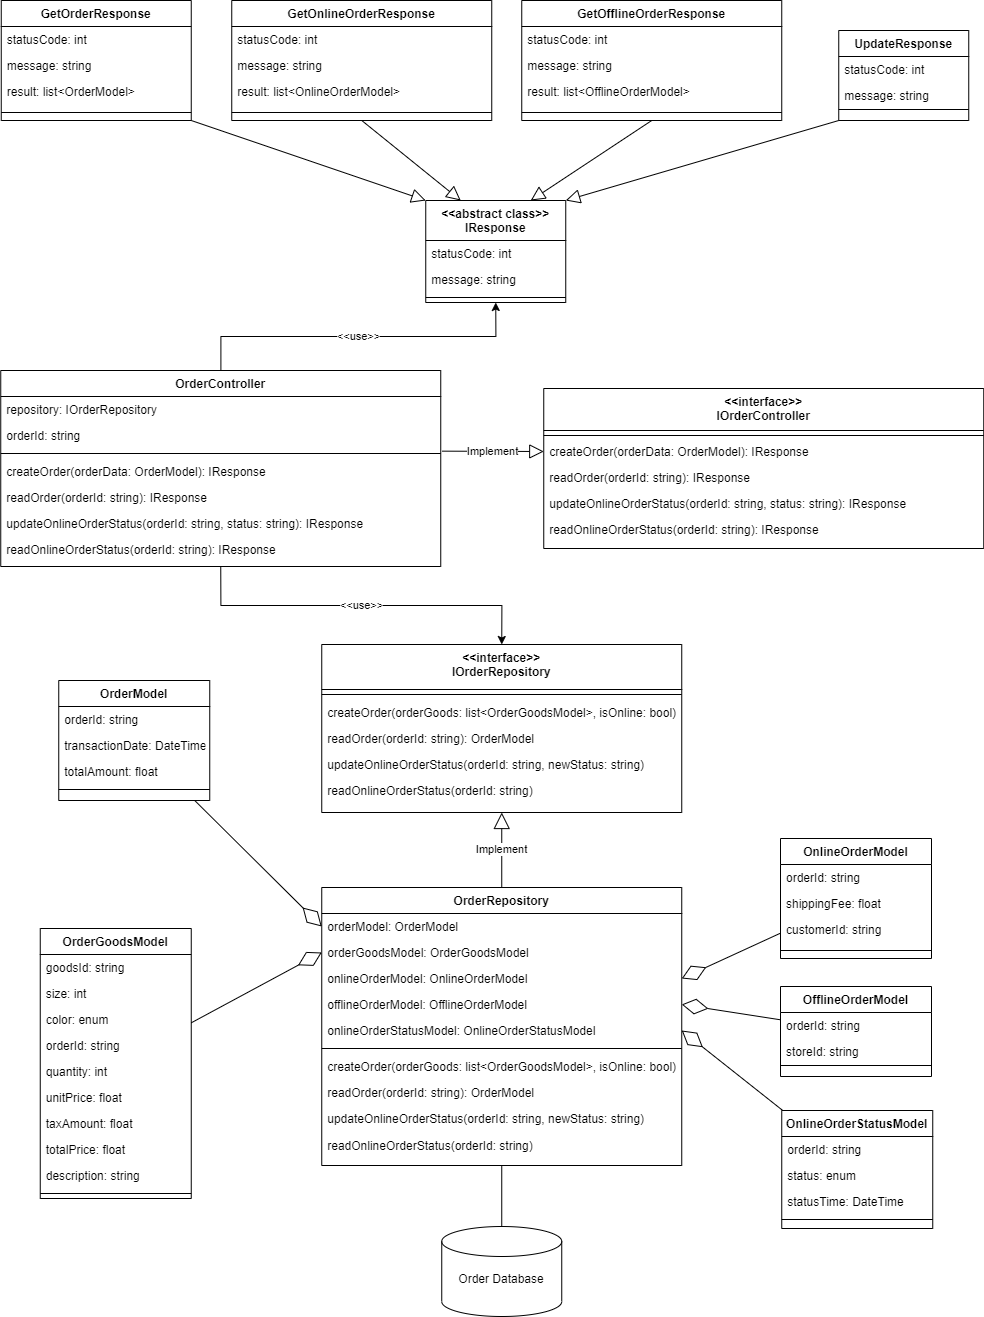
\includegraphics[width=11cm]{img/Architecture/service/OrderService.png}
	\newline
	\caption{Lược đồ class của Order Service}
\end{figure}



\subsubsection{Account Service}
\begin{figure}[!htp]
	\centering
	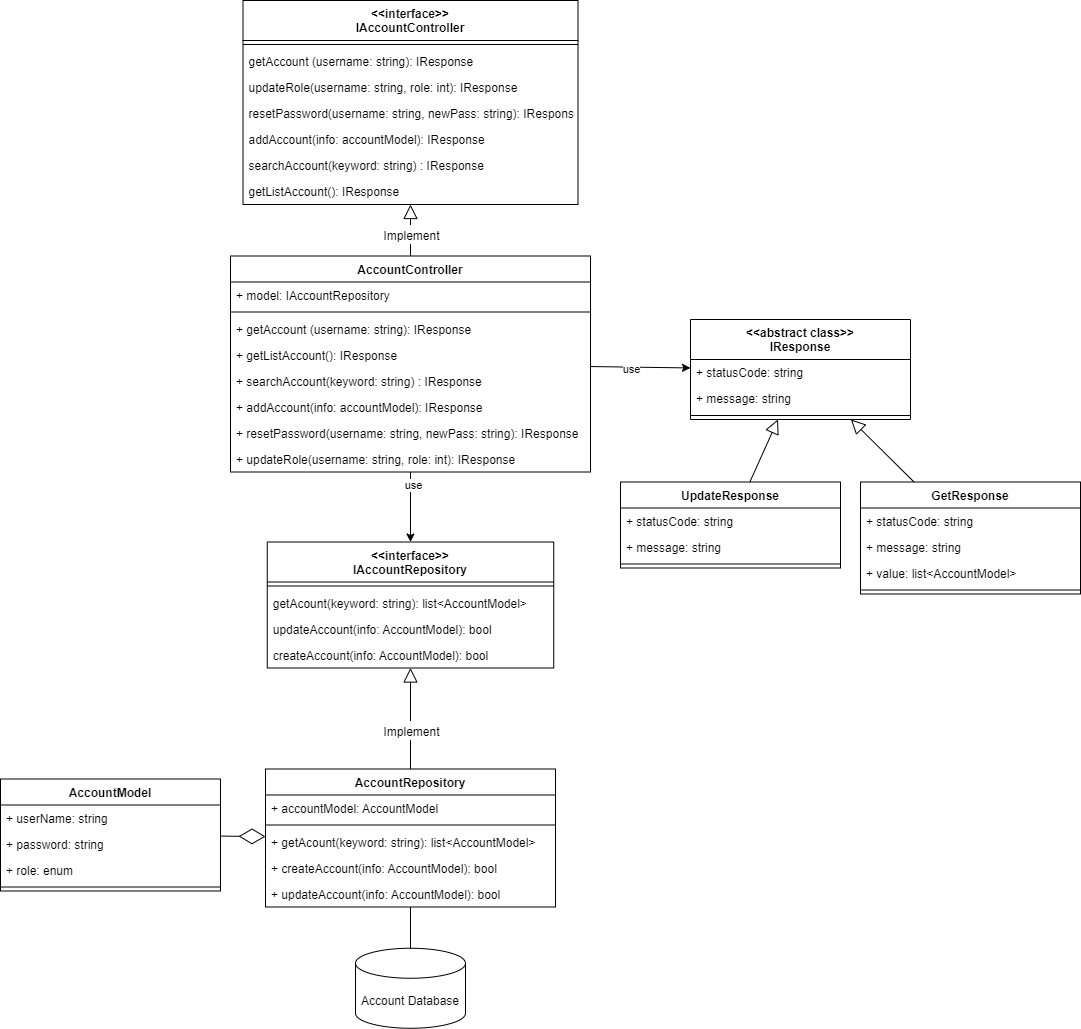
\includegraphics[width=11cm]{img/Architecture/service/AccountService.png}
	\newline
	\caption{Lược đồ class của Account Service}
\end{figure}



\subsubsection{Staff Service}
\begin{figure}[!htp]
	\centering
	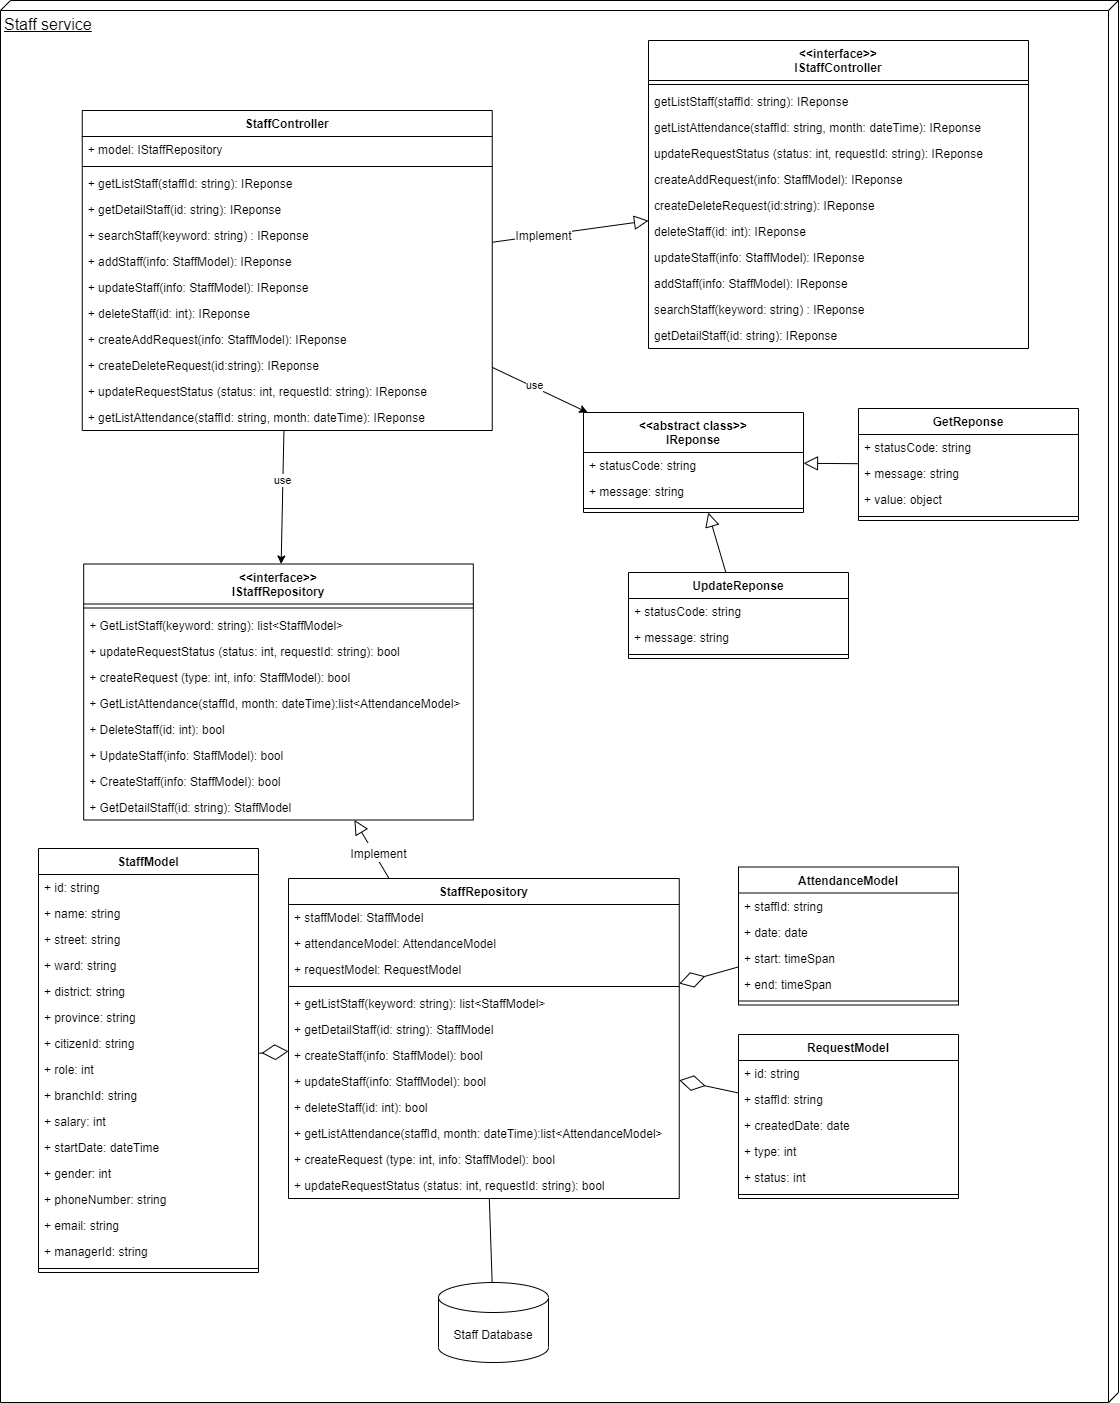
\includegraphics[width=11cm]{img/Architecture/service/StaffService.png}
	\newline
	\caption{Lược đồ class của Staff Service}
\end{figure}



\subsubsection{Branch Service}
\begin{figure}[!htp]
	\centering
	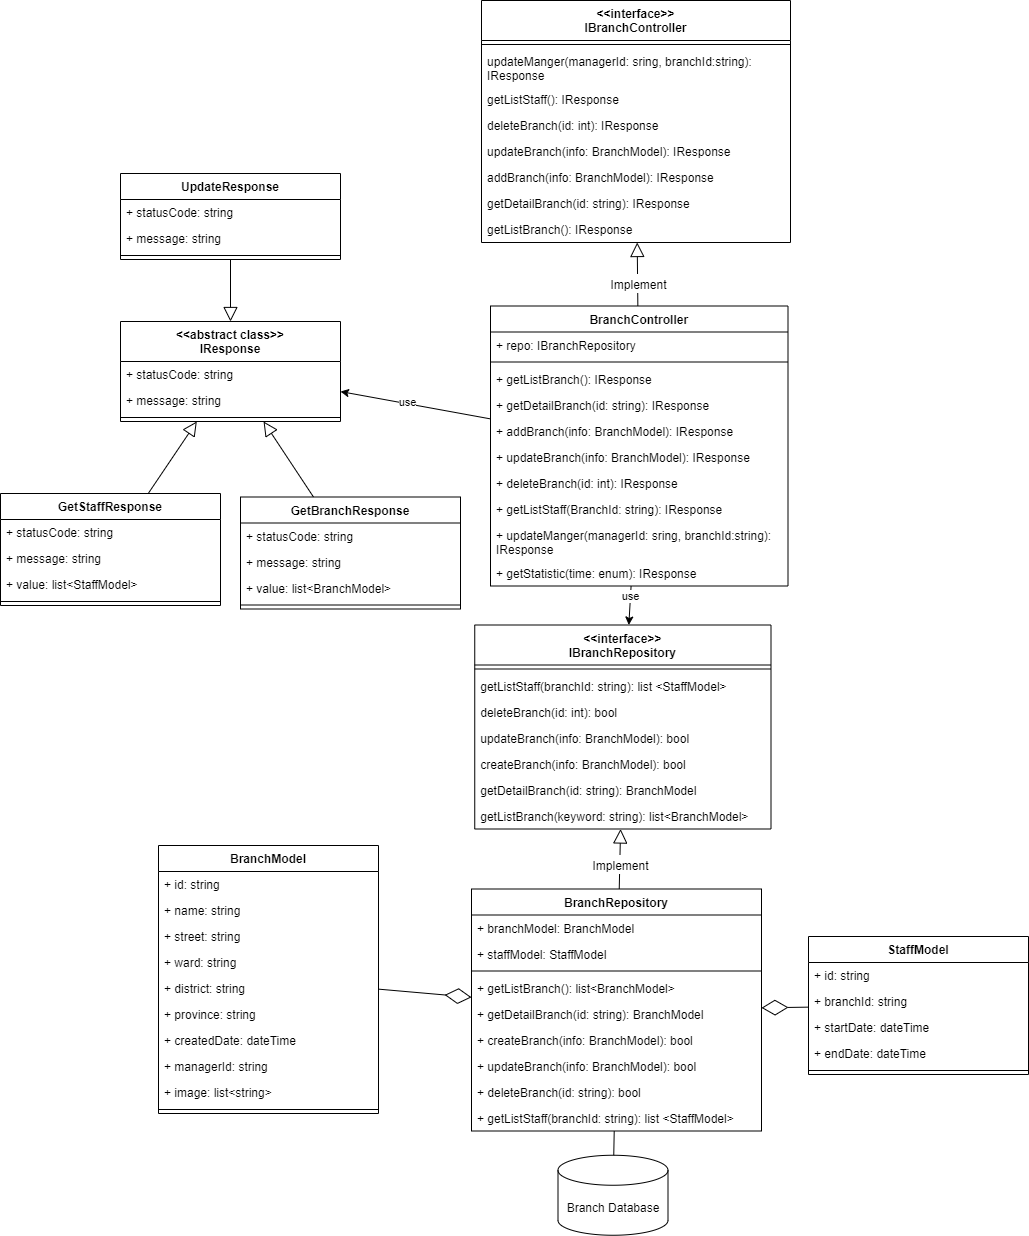
\includegraphics[width=10cm]{img/Architecture/service/BranchService.png}
	\newline
	\caption{Lược đồ class của Branch Service}
\end{figure}

\subsubsection*{BranchRepository}
Thuộc tính:
\begin{itemize}
	\item branchModel: Chứa đối tượng BranchModel
	\item staffModel: Chứa đối tượng StaffModel
\end{itemize}
Phương thức:
\begin{itemize}
	\item getListBranch(): Lấy danh sách chi nhánh
	\item getDetailBranch(id: string): Lấy thông tin chi tiết một chi nhánh
	\item createBranch(info: BranchModel): Thêm một chi nhánh mới
	\item updateBranch(info: BranchModel): Cập nhật thông tin một chi nhánh
	\item deleteBranch(id: string): Xóa một chi nhánh
	\item getListStaff(BranchId: string): Lấy danh sách nhân viên của chi nhánh
\end{itemize}

\subsubsection*{BranchModel}
Thuộc tính:
\begin{itemize}
	\item id: Id của chi nhánh
	\item name: Tên của chi nhánh
	\item street: Tên đường của chi nhánh
	\item ward: Phường của chi nhánh
	\item province: Tỉnh của chi nhánh
	\item createdDate: Ngày tạo chi nhánh
	\item managerId: Id của người quản lý
	\item image: Các hình ảnh của chi nhánh
\end{itemize}

\subsubsection*{StaffModel}
Thuộc tính:
\begin{itemize}
	\item id: Id của nhân viên
	\item branchId: Id của chi nhánh làm việc
	\item startDate: Thời gian bắt đầu làm việc tại chi nhánh
	\item endDate: Thời gian kết thúc làm việc tại chi nhánh
\end{itemize}

\subsubsection*{BranchController}
Thuộc tính:
\begin{itemize}
	\item repo: Chứa đối tượng repository
\end{itemize}
Phương thức:
\begin{itemize}
	\item getListBranch(): Lấy danh sách chi nhánh
	\item getDetailBranch(id: string): Lấy thông tin chi tiết một chi nhánh
	\item addBranch(info: BranchModel): Thêm một chi nhánh mới
	\item updateBranch(info: BranchModel): Cập nhật thông tin một chi nhánh
	\item deleteBranch(id: int): Xóa một chi nhánh
	\item getListStaff(BranchId: string): Lấy danh sách nhân viên của chi nhánh
	\item updateManger(managerId: sring, branchId:string): Cập nhật quản lý chi nhánh
	\item getStatistic(time: enum): Lấy thông tin thống kê lợi nhuận, doanh thu.
\end{itemize}

\subsubsection*{UpdateResponse - GetStaffResponse - GetBranchResponse }
Thuộc tính:
\begin{itemize}
	\item statusCode: Mã trạng thái của phản hồi
	\item message: Thông điệp của phản hồi
	\item value: Các dữ liệu trả về đối với các yêu cầu HTTP GET
\end{itemize}



\subsubsection{Event Service}
\begin{figure}[!htp]
	\centering
	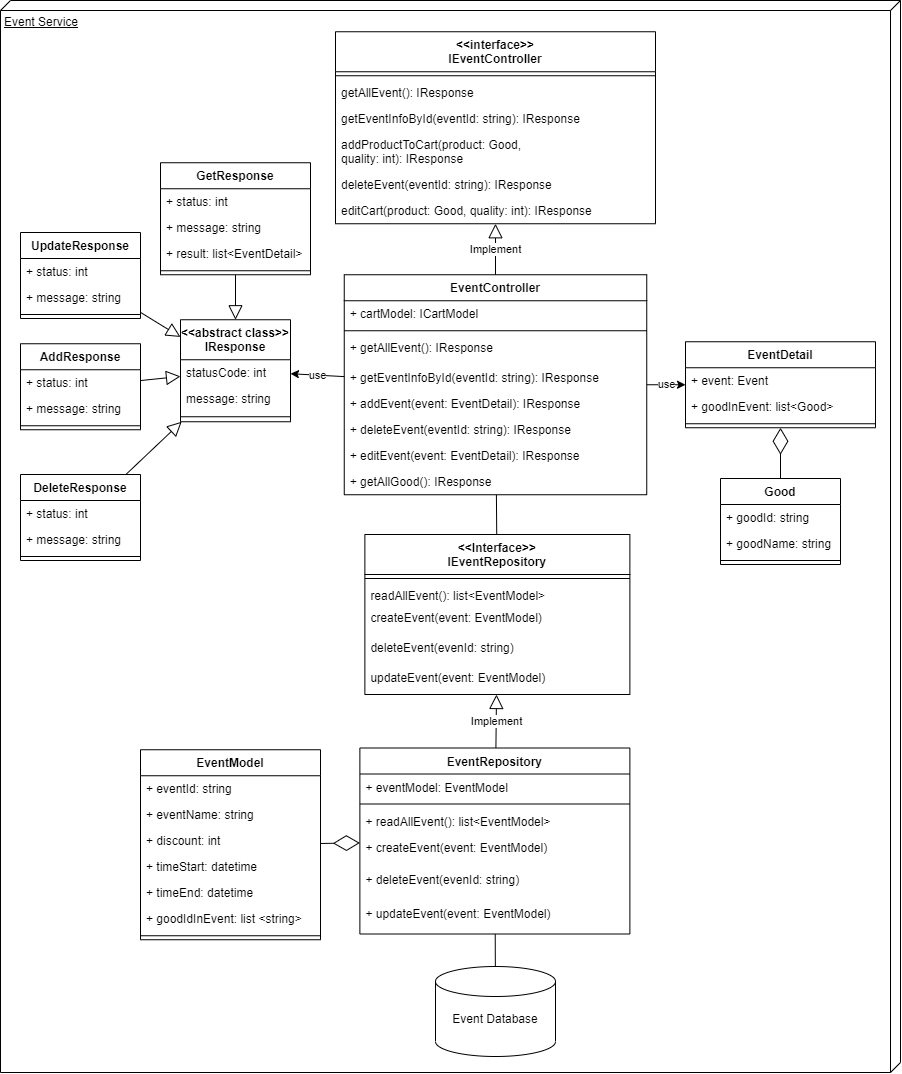
\includegraphics[width=11cm]{img/Architecture/service/EventService.png}
	\newline
	\caption{Lược đồ class của Event Service}
\end{figure}


\subsubsection{Warehouse Service}
\begin{figure}[!htp]
	\centering
	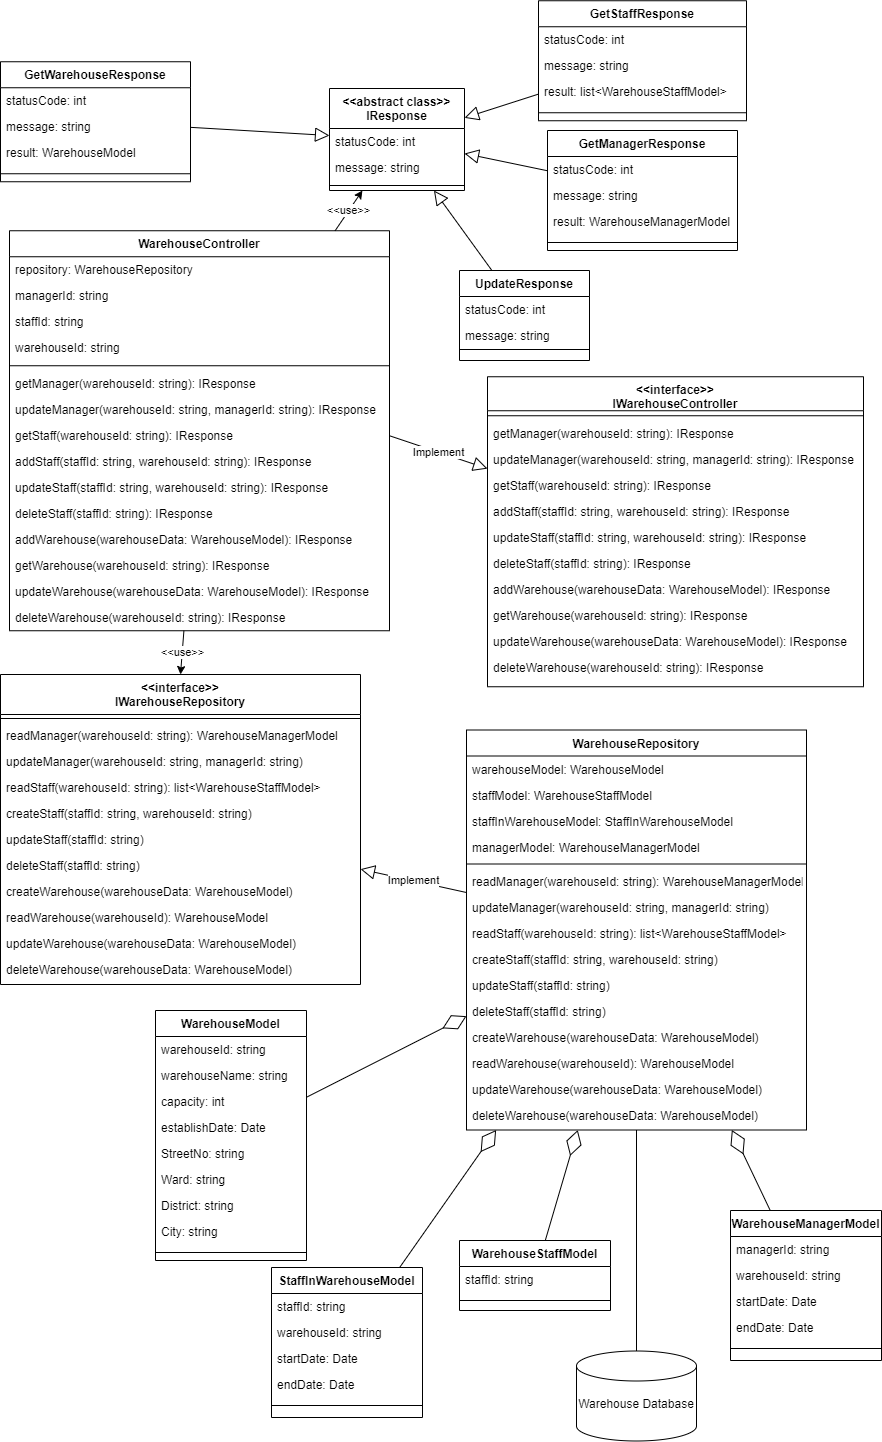
\includegraphics[width=11cm]{img/Architecture/service/WarehouseService.png}
	\newline
	\caption{Lược đồ class của Warehouse Service}
\end{figure}


\subsubsection{Statistic Service}
\begin{figure}[!htp]
	\centering
	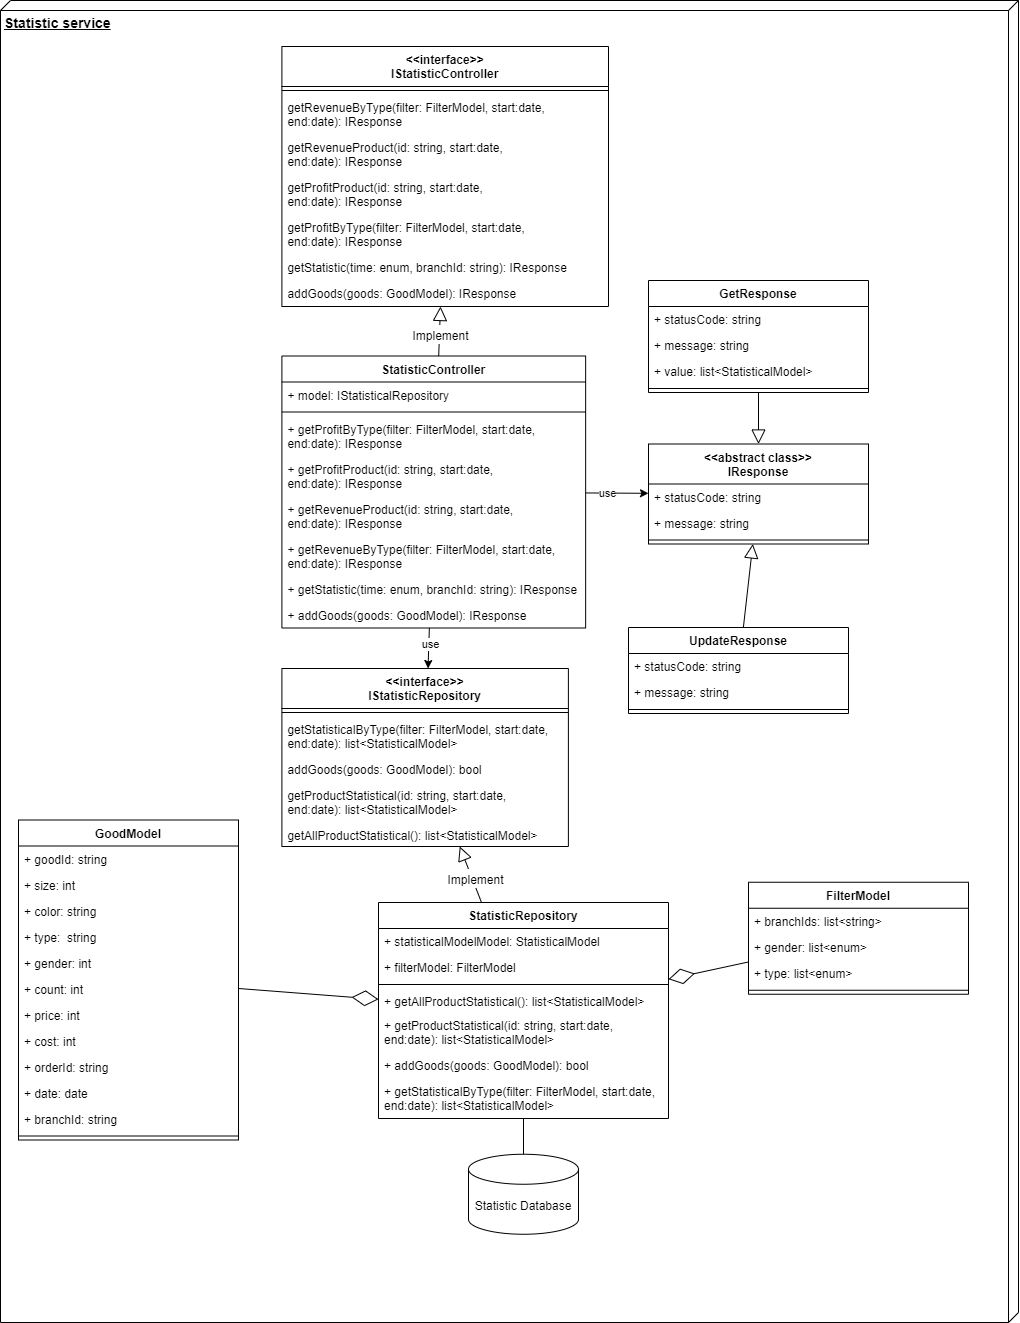
\includegraphics[width=11cm]{img/Architecture/service/StatisticService.png}
	\newline
	\caption{Lược đồ class của Statistic Service}
\end{figure}
\textbf{Mô tả:}
\begin{quote}
	\begin{itemize}
		\item ...
		\item ...
	\end{itemize}
\end{quote}

\subsubsection{Goods Service}
\begin{figure}[!htp]
	\centering
	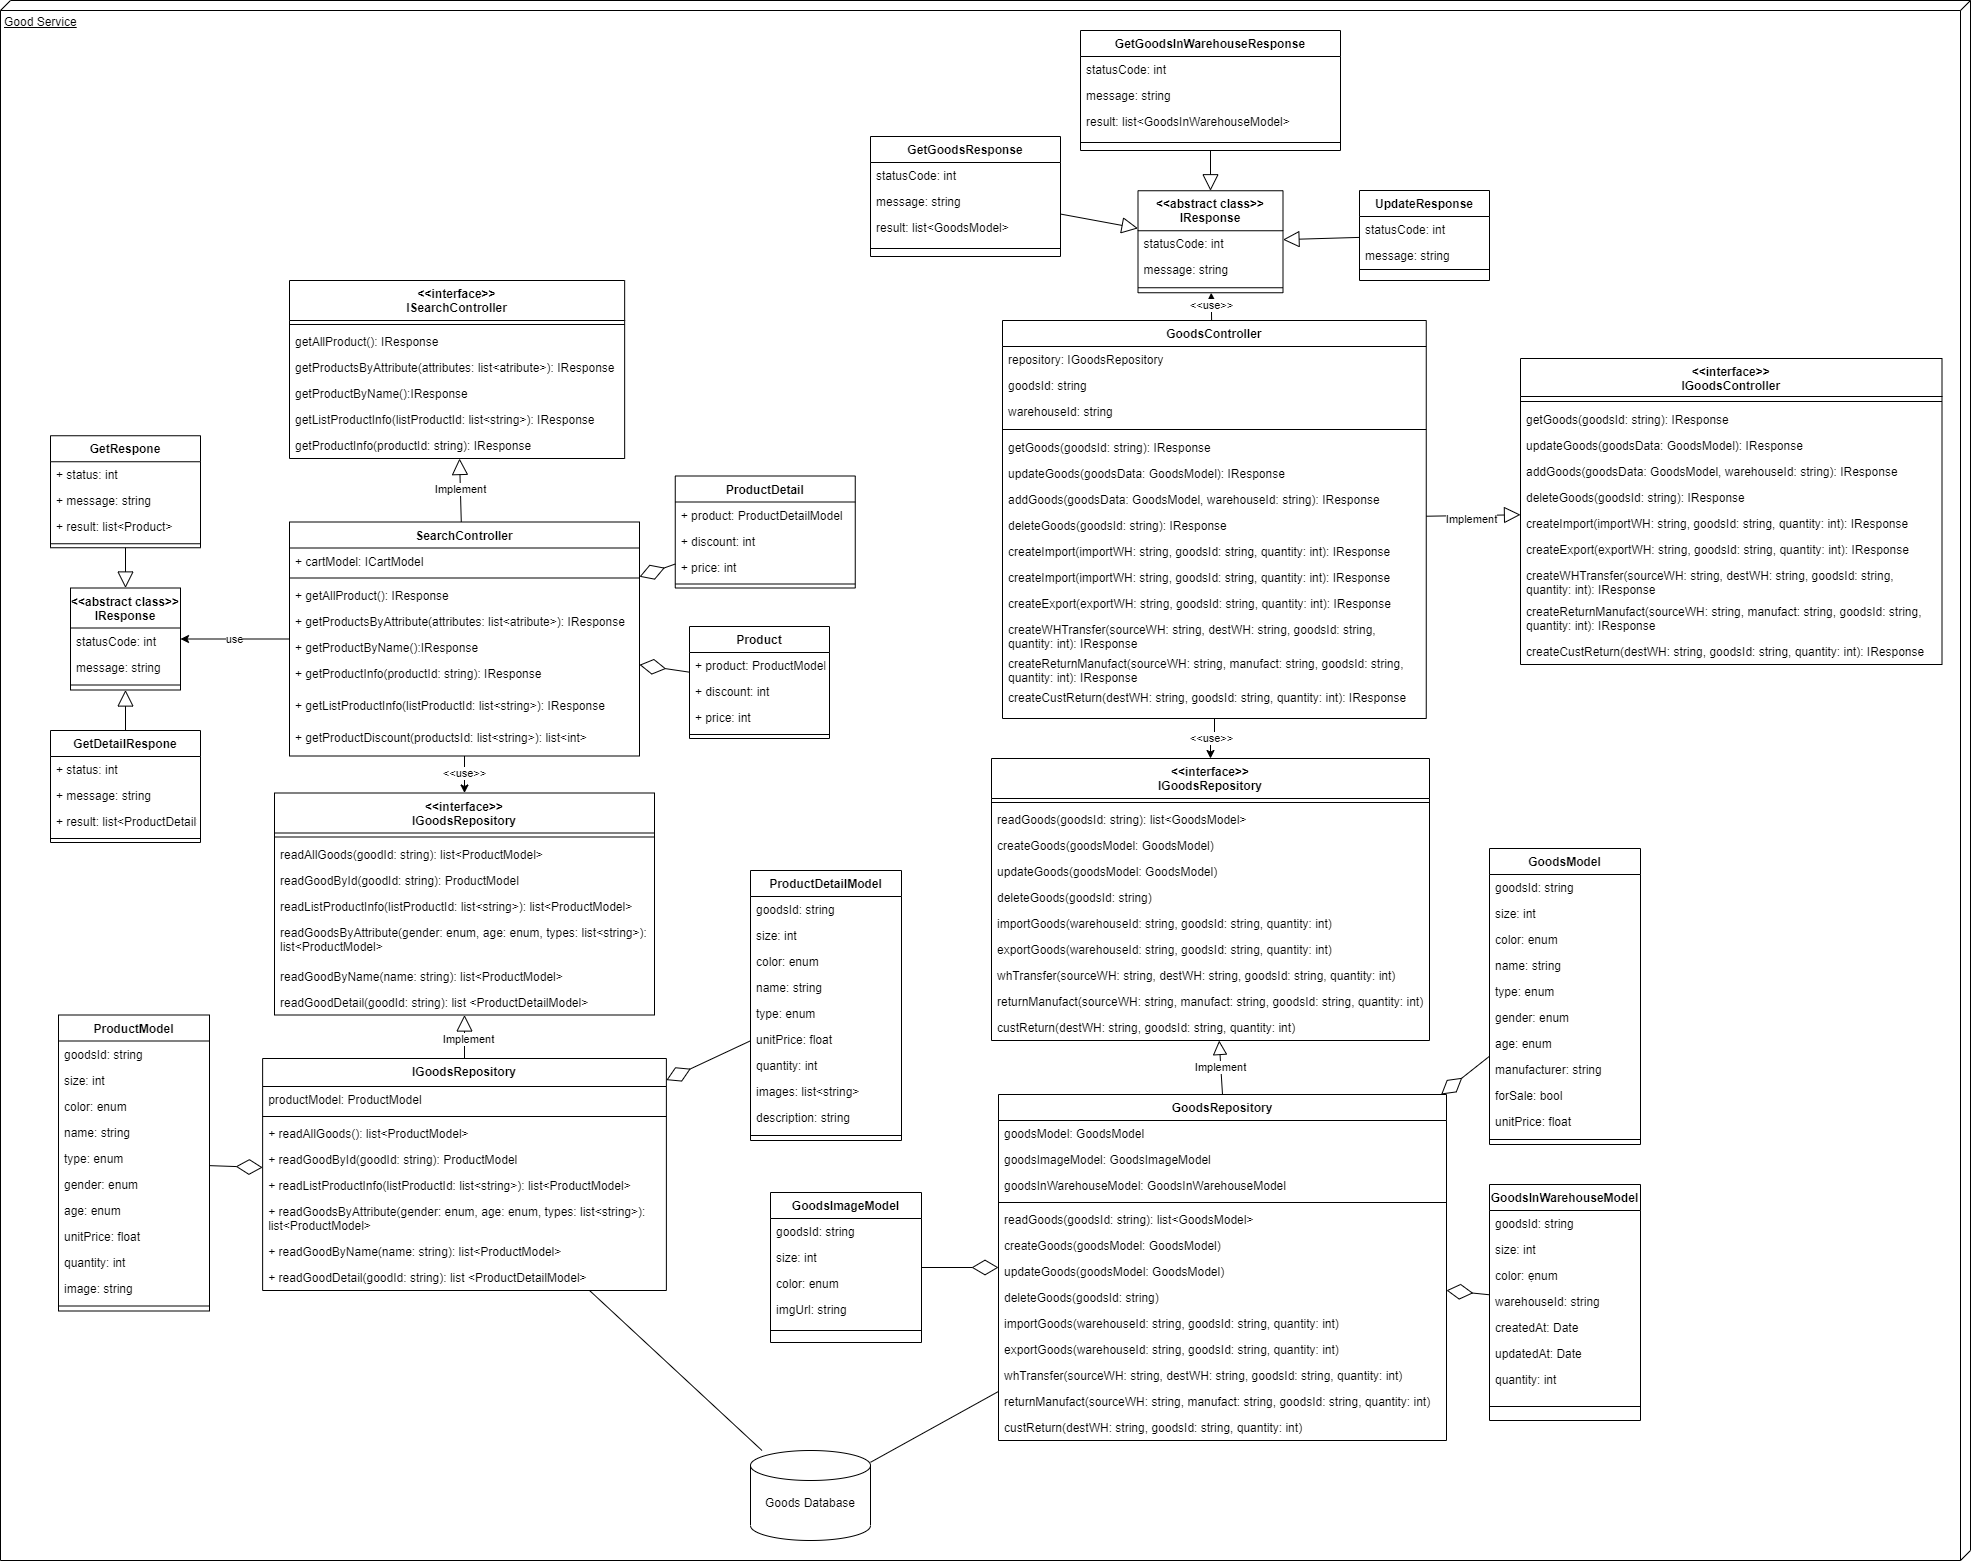
\includegraphics[width=17cm]{img/Architecture/service/GoodsService.png}
	\newline
	\caption{Lược đồ class của Goods Service}
\end{figure}

